% ****** Start of file apssamp.tex ******
%
%   This file is part of the APS files in the REVTeX 4.2 distribution.
%   Version 4.2a of REVTeX, December 2014
%
%   Copyright (c) 2014 The American Physical Society.
%
%   See the REVTeX 4 README file for restrictions and more information.
%
% TeX'ing this file requires that you have AMS-LaTeX 2.0 installed
% as well as the rest of the prerequisites for REVTeX 4.2
%
% See the REVTeX 4 README file
% It also requires running BibTeX. The commands are as follows:
%
%  1)  latex apssamp.tex
%  2)  bibtex apssamp
%  3)  latex apssamp.tex
%  4)  latex apssamp.tex


\documentclass[%
 reprint,
%superscriptaddress,
%groupedaddress,
%unsortedaddress,
%runinaddress,
%frontmatterverbose, 
%preprint,
%preprintnumbers,
nofootinbib,
%nobibnotes,
%bibnotes,
 amsmath,amssymb,
 aps,
%pra,
%prb,
%rmp,
%prstab,
%prstper,
%floatfix,
]{revtex4-2}

% \documentclass[reprint, amsmath, amssymb, aps, twocolumn]{article}


\usepackage{graphicx}% Include figure files
\usepackage{dcolumn}% Align table columns on decimal point
\usepackage{bm}% bold math
\usepackage[english]{babel}
\usepackage{lipsum}
\usepackage{amsmath}
\usepackage{float}
\usepackage{physics}
% \usepackage[style=phys,articletitle=false,biblabel=brackets,
% chaptertitle=false,pageranges=false]{biblatex}
  %AIP/APS style
\usepackage{appendix}

%\addbibresource{apssamp.bib} %Imports bibliography file

%\usepackage{hyperref}% add hypertext capabilities
%\usepackage[mathlines]{lineno}% Enable numbering of text and display math
%\linenumbers\relax % Commence numbering lines

%\usepackage[showframe,%Uncomment any one of the following lines to test 
%%scale=0.7, marginratio={1:1, 2:3}, ignoreall,% default settings
%%text={7in,10in},centering,
%%margin=1.5in,
%%total={6.5in,8.75in}, top=1.2in, left=0.9in, includefoot,
%%height=10in,a5paper,hmargin={3cm,0.8in},
%]{geometry}

\begin{document}
% \addbibresource{apssamp.bib} %Imports bibliography file
% \preprint{APS/123-QED}

\title{Strain Engineering and Dissipation Dilution for a Room-Temperature Spin-Optomechanical Transducer}% Force line breaks with \\
%A Review of Dissipation Dilution and Strain Engineering \\ as Relevant to Cavity Optomechanics
% \thanks{A footnote to the article title}%

\author{Ruchir Tullu}
 \altaffiliation{University of Toronto}%Lines break automatically or can be forced with \\
% \author{Second Author}%
\email{\\ruchir.tullu@mail.utoronto.ca}
% \affiliation{%
%  Authors' institution and/or address\\
%  This line break forced with \textbackslash\textbackslash
% }%

% \collaboration{MUSO Collaboration}%\noaffiliation

% \author{Charlie Author}
%  \homepage{http://www.Second.institution.edu/~Charlie.Author}
% \affiliation{
%  Second institution and/or address\\
%  This line break forced% with \\
% }%
% \affiliation{
%  Third institution, the second for Charlie Author
% }%
% \author{Delta Author}
% \affiliation{%
%  Authors' institution and/or address\\
%  This line break forced with \textbackslash\textbackslash
% }%

% \collaboration{CLEO Collaboration}%\noaffiliation

\date{\today}% It is always \today, today,
             %  but any date may be explicitly specified

\begin{abstract}
In this report we discuss the effects of dissipation dilution and strain engineering as relevant to cavity optomechanics. We begin by discussing basic optomechanics theory, then review strain engineering and dissipation dilution. Finally, we present some numerical simulation results done in \textit{COMSOL Multiphysics} to simulate the effects of dissipation dilution and strain engineering in mechanical resonators. We also present some alternative resonator designs and their advantages/disadvantages over the tapered PnC design. The results obtained in COMSOL show signs of approaching the mode shape required, however more work is required for this to accurately represent the mode shape obtained by Ghadimi et al. for the tapered PnC nanobeams.

% The quality factor of a tapered PnC resonator was found to be $\sim 10^7$

% We note that such resonators may be used ubiquitously for a variety of applications, from fundamental tests of quantum mechanics, to extremely sensitive force detectors, to being used in quantum technologies.

% \begin{description}
% \item[Usage]
% Secondary publications and information retrieval purposes.
% \item[Structure]
% You may use the \texttt{description} environment to structure your abstract;
% use the optional argument of the \verb+\item+ command to give the category of each item. 
% \end{description}
\end{abstract}

%\keywords{Suggested keywords}%Use showkeys class option if keyword
                              %display desired
\maketitle

%\tableofcontents

\section{Introduction}

Quantum networks allow for the transmission of quantum information (qubits) over distant locations, or nodes. These networks take advantage of quantum mechanical phenomenon to provide more secure information exchange than is possible in classical communication networks. These networks will enable key applications, including quantum key distribution, a quantum internet, fundamental tests of quantum gravity and quantum mechanics, among others \cite{project_paper}. However, due to various loss mechanisms when transmitting quantum information over sufficiently large distance scales (i.e. decoherence), the need for a quantum repeater arises. These repeaters provide a way for the qubits to be stored in quantum memories, and are subsequently re-emitted as photonic qubits for further use, thereby preserving the quantum information. One such component of these repeaters is known as a quantum transducer; these provide a means of energy transfer, or more fundamentally, information transfer between two states. 
\newline 

Elastic strain engineering has provided a promising range of possibilities with respect to nano-scale materials. The tuning of the elastic strain field allows for the tuning of physical properties of a system, leading to novel new applications of this phenomenon \cite{elastic_strain_engineering}. Within the context of strain engineering, there emerges a new way to limit the dissipation of a mechanical resonator by tuning the static and elastic strain. This gives rise to higher mechanical quality factors, and enhanced $Qf$ products for mechanical resonators.
\newline

In this report we discuss the relevance of strain engineering and dissipation dilution in the context of cavity optomechanics. We apply these principles to simulations in COMSOL Multiphysics to test the properties of these strain engineered resonators. Finally, we conclude by discussing some alternative designs.


% \subsection{Quantum Networks and Quantum Repeaters}

% Quantum networks are an upcoming technology


% \begin{figure*}[htb]
%     \centering
%     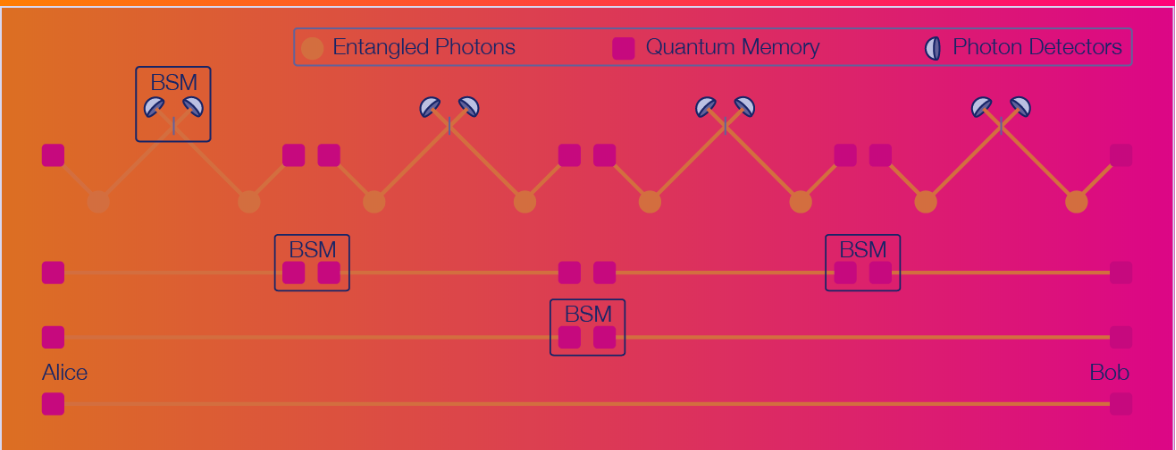
\includegraphics [width=\textwidth, height=7.5cm] {Quantum_Repeaters.PNG}
%     \caption{Quantum Repeater \textbf{REFERENCE}}
%     \label{fig:Quantum Repeater}
% \end{figure*}


\section{\label{sec:level1}Review of Basic Optomechanics Theory:}

\subsection{Mechanical Resonators}

Mechanical resonators are ubiquitous tools in modern-day science and engineering, with applications ranging from silicon chip technologies to gravitational wave interferometers. The use of mechanical resonators in quantum technologies has brought with it novel ways to detect quantum phenomenon, including accurate detection of small-scale forces and usage in hybrid transducer systems. Here we review some theory behind mechanical resonators and discuss their implications.

\subsubsection{Euler-Bernoulli Beam Theory}
One may solve for the vibrational modes $u_{n}(x)$ of an oscillator of arbitrary geometry by solving the appropriate equations of the linear theory of elasticity subject to the proper boundary conditions. One then obtains a set of normal modes and their corresponding eigenfrequencies \cite{cavity_optomechanics_2014}. The Euler-Bernoulli beam equations are a simplification to the linear theory of elasticity:

\begin{equation*}   % * suppresses numbering in amsmath package
    \frac{d^2}{dx^2} \Big( EI \frac{d^2u}{dx^2} \Big) = q
\end{equation*}


\begin{equation*}   % * suppresses numbering in amsmath package
    \frac{\partial^2}{\partial x^2} \Big( EI \frac{\partial^2u}{\partial x^2} \Big) = -\mu \frac{\partial^2 u}{\partial t^2} + q(x)
\end{equation*}
% \newline

With the former equation being for the static beam case, and the latter equation being for the dynamic beam case. Here, $E$ represents the elastic modulus of the material, $I$ represents the second moment of area, $q$ represents the external load, and $\mu$ represents the mass per unit length.


\subsubsection{Classical Resonators}

The canonical equation of motion describing a mechanical resonator with effective mass  $m_{eff}$ \footnote{Note that comparing the value of [\ref{Vibrational Energy}] to the value for the potential energy given by the linear theory of elasticity, one is able to find the correct value of $m_{eff}$.} and global displacement $x(t)$ can be written as follows:

\begin{equation} \label{Harmonic Oscillator Equation}
    m_{eff}\frac{d^2 x(t)}{dt^2} + m_{eff}\Gamma_{m}\frac{dx(t)}{dt} + m_{eff}\Omega_{m}^2 x(t) = F_{ex}(t)
\end{equation}

Where $\Omega_{m}$ is the mechanical frequency of vibration, $\Gamma_{m}$ is the energy damping rate, and $F_{ex}$ is the total external force applied to the resonator. $\Gamma_{m}$ is related to the resonator quality factor, $Q_{m}$, by $\Gamma_{m} = \frac{\Omega_{m}}{Q_{m}}$. The quality factor is a term that characterizes the energy loss of the resonator. It may be defined as:

$$Q_{m} \triangleq 2\pi \frac{W}{\Delta W}$$

Where $W$ is the total energy stored in the resonator, and $\Delta W$ is the energy lost per oscillation period. Alternatively, one may also define $Q_{m}$ as:

$$ Q_{m} \equiv \frac{\Omega_{m}}{\Gamma_{m}} $$

Therefore, a quality factor much greater than unity means an oscillator with minimal losses in vibrational energy. One may write the elastic potential energy of a mechanical resonator as:

\begin{equation} \label{Vibrational Energy}
    E_{vibrational} = \frac{m_{eff}\Omega_{m}^2 \big \langle x(t) \big \rangle ^2}{2}
\end{equation}

Where $\big \langle \boldsymbol{\cdot} \big \rangle $ denotes a time averaged value. We may visualize a solution to (\ref{Harmonic Oscillator Equation}) in Figure \ref{fig:mechanical_oscillator}:

\begin{figure}[htb]
    \centering
    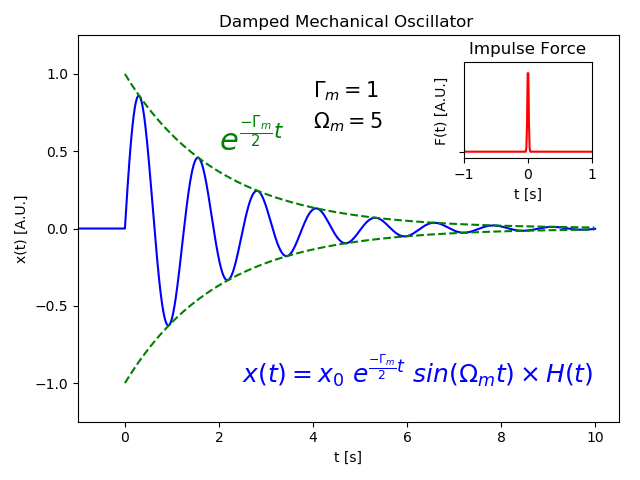
\includegraphics [width=\columnwidth, height=7.5cm] {damped_mechanical_oscillator.png}
    \caption{Damped Mechanical Oscillator. The chosen parameters result in a decaying global displacement $x(t)$. The inset shows the impulse force applied at $t = 0$. The function $H(t)$ multiplying the global amplitude of the resonator denotes the Heaviside step function. }
    \label{fig:mechanical_oscillator}
\end{figure}

% \newpage
\subsubsection{Quantum Mechanical Treatment of Mechanical Resonators}

The quantum mechanical treatment of the mechanical resonator leads to the following Hamiltonian \cite{cavity_optomechanics_2014}:

\begin{equation} \label{Mechanical Resonator Hamiltonian}
    \hat{H} = \hbar \Omega_{m} \hat{b}^{\dagger}\hat{b} + \frac{1}{2} \hbar \Omega_{m}
\end{equation}

Where $\hat{b}^{\dagger}$ and $\hat{b}$ represent the phonon creation and annihilation operators, respectively. The position and momentum of the mechanical resonator are given by:

\centering
$$ \hat{x} = x_{zpf} \big( {\hat{b} + \hat{b}^{\dagger}} \big)$$ 
$$\hat{p} = -i m_{eff} \Omega_{m} x_{zpf} \big( {\hat{b} - \hat{b}^{\dagger}} \big)$$

\flushleft
Where 

$$ x_{zpf} = \sqrt{\frac{\hbar}{2m_{eff}\Omega_{m}}} $$
\

represents the \textit{zero point fluctuation amplitude} of the mechanical resonator. $x_{zpf}$ can also be expressed as:
\

$$ x_{zpf}^2 = \expval{\hat{x}^2}{0} $$     % Braket notation
\

Where $\mid{0} \big \rangle$ denotes the mechanical vacuum state. The zero point fluctuation is important for optomechanical experiments, as a mechanical resonator close to it's $x_{zpf}$ will display quantum mechanical effects.
\newline

The thermal decoherence rate of a mechanical oscillator is given as:

$$\frac{k_{B}T_{bath}}{\hbar Q_{m}} $$

Where $k_{B}$ is Boltzmann's constant, and $T_{bath}$ is the temperature of the bath the mechanical resonator is coupled to. The thermal decoherence rate describes the rate at which the oscillator heats out of the ground state. 


\subsubsection{Mechanical Dissipation $\&$ Loss Mechanisms in Nanomechanical Resonators}
Mechanical resonators lose energy at the energy dissipation rate of $\Gamma_m = \Omega_m / Q_m$. This quantity corresponds to the loss of mechanical excitations, or phonons. The relevant loss mechanisms that have been studied so far are as follows \cite{cavity_optomechanics_2014}:

\begin{itemize}

    \item \textit{Viscous damping} \\
        Caused by the interactions of surrounding gas atoms or compression of thin fluidic layers
        
    \item \textit{Clamping losses} \\
       Due to the radiation of elastic waves into the the substrate through the supports of the oscillator
        
    \item \textit{Thermoelastic damping/ phonon-phonon interactions} \\
        These are fundamental anharmonic effects. Thermoelastic damping can be thought of as irreversible heat flow from regions of higher strain (having higher temperature) to regions of lower strain (having lower temperature), resulting in a loss of energy.
        
    \item \textit{Material-induced losses} \\
       Caused by the relaxation of intrinsic or extrinsic defect states in the resonator. These have been described by two-level defect models \cite{two_level_damping}.

\end{itemize}


The various loss mechanisms result in independent contributions to the quality factor as \cite{cavity_optomechanics_2014, ghadimi_thesis}:

\begin{equation*}
    \frac{1}{Q_{total}} = \sum \frac{1}{Q_i}
\end{equation*}

Where $i$ indexes the different loss mechanisms. An important figure of merit for mechanical oscillators in the context of optomechanics is the $Qf$ product. This quantifies the decoupling of the oscillator from the thermal environment. In particular, the expression

\begin{equation}\label{eq:coherent_oscillations}
    \frac{\Omega_m}{\bar{n}_{th} \Gamma_m} = Q_m f_m \times \Big ( \frac{h}{k_B T} \Big )
\end{equation}

denotes the number of coherent oscillations of the oscillator in the presence of thermal decoherence; this scales as $Q_m f_m$ \cite{cavity_optomechanics_2014}.
\newline

In particular, for nanobeam resonoators at high $Q$-factors, two dominant loss mechanisms are gas damping and surface losses \cite{Surface_losses}. These are both addressed in \cite{ [{pg. 34, 175}] ghadimi_thesis}, pg. 34, 175.


\subsection{Optical Cavities}

Optical cavities are a system of mirrors designed to produce standing mode resonances of light reflecting inside them. The light sent into the cavity will experience interference, resulting in standing waves at particular frequencies, depending on the length of the cavity. These systems often have very large quality factors, meaning little attenuation of the input signal. One such example of an optical cavity is the Fabry-P\'{e}rot resonator.


\subsubsection{Fabry-P\'{e}rot  Resonators}

Fabry-P\'{e}rot resonators are a simple example of an optical cavity. They consist of two reflective mirrors seperated by a distance $L$ which contain the optical modes in between them. Light is able to reflect within this cavity and form certain resonant modes (as in Figure \ref{fig:Fabry-Perot Cavity}).


\begin{figure}[htb]
    \centering
    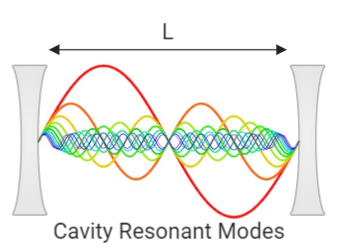
\includegraphics [width=\columnwidth, height=5.5cm]{Fabry-Perot_Interferometer.PNG}
    \caption{Illustration of Fabry-P\'{e}rot  cavity resonances (optical modes).}
    \label{fig:Fabry-Perot Cavity}
\end{figure}


The resonant modes produced in the Fabry-P\'{e}rot cavity have angular frequencies given by $\omega_{cav,m} = m \frac{\pi c}{L}$, where $m$ is the mode number. These angular frequencies are separated between two longitudinal modes by the \textit{free spectral range} (FSR) of the cavity:

\begin{equation*}
   \Delta \omega_{FSR} = \frac{\pi c}{L}
\end{equation*}

Natural imperfections in the optical cavity system, such as internal absorption, finite mirror transparencies, or scattering of light out of the cavity leads to a finite photon (intensity) cavity decay rate, $\kappa$. We may define the optical \textit{finesse} of the cavity as follows:

\begin{equation*}
    \mathcal{F} \equiv \frac{\Delta \omega_{FSR}}{\kappa}= \frac{\pi c}{L \kappa}
\end{equation*}

This quantity defines the average number of trips before a photon leaves the cavity. Related to the finesse, the optical quality factor can be defined as:

\begin{equation*}
    Q_{opt} = \omega_{cav}\tau
\end{equation*}

Where $\tau = 1/\kappa$ is the photon lifetime. We may model the loss from a high-Q cavity as:

\begin{equation*}
    \kappa = \kappa_{ex} + \kappa_{0}
\end{equation*}

Where $\kappa_{ex}$ refers to the loss associated with the input coupling, and $\kappa_{0}$ refers to any remaining loss rate \cite{cavity_optomechanics_2014}. 

\subsubsection{Input-Output Formalism}

Here we briefly touch on some concepts of the input-output formalism for optical cavities as presented in \cite{cavity_optomechanics_2014}. The interested reader is referred to other sources for more detailed information \cite{cavity_optomechanics_2014}.
\newline

Quantum mechanical descriptions of open systems such as optical cavities coupled to the outside electromagnetic field can be done through the usage of master equations, or input-output theory. The former is useful if internal dynamics are of the main concern, but input-output theory also takes into account the light field being emitted or reflected from the cavity.
\newline

There exists some field amplitude $\hat{a}$ inside the optical cavity which experiences a decay rate of $\kappa /2$, but is also replenished by quantum noise entering the system via various ports in the cavity. The dynamics of this system can be described by the equation of motion:

\begin{equation}\label{eq:equation_of_motion_cavity}
    \dot{\hat{a}} = -\frac{\kappa}{2}\hat{a} + i\Delta\hat{a} + \sqrt{\kappa_{ex}}\hat{a}_{in} + \sqrt{k_{0}}\hat{f}_{in}
\end{equation}

Here, $\hat{a}_{in}$ represents a stochastic quantum field. It can be as simple as the sum of the fluctuating vacuum electric field coupling to the cavity, plus a coherent laser drive, or as complicated as needed. The input power into the cavity can be written as:

\begin{equation}\label{eq:Power_eq}
    P = \hbar \omega_{L} \big < \hat{a}_{in}^{\dagger} \hat{a}_{in} \big >
\end{equation}

Note that the field normalization is chosen such that $\big < \hat{a}_{in}^{\dagger} \hat{a}_{in} \big >$ represents the rate of photons arriving in the cavity (and $\omega_{cav} \approx \omega_{L}$). The same description may be applied as above to any unwanted channels as given by $\hat{f}_{in}$.
\newline

The field reflected from a Fabry-P\'{e}rot resonator as given by input-output theory is given by:

\begin{equation*}
    \hat{a}_{out} = \hat{a}_{in} - \sqrt{\kappa_{ex}} \hat{a}
\end{equation*}

The solution of (\ref{eq:equation_of_motion_cavity}) for steady-state amplitude in the presence of a monochromatic laser drive whose amplitude is given by $\big < \hat{a}_{in} \big >$ is as follows:

\begin{equation*}
    \big < \hat{a} \big > = \frac{\sqrt{\kappa_{ex}}\big < \hat{a}_{in} \big >}{\frac{\kappa}{2} - i\Delta}
\end{equation*}

Here we note that $\big< \hat{f}_{in} \big > = 0$.
\newline

The steady state cavity population is given by:

\begin{equation*}
    \bar{n}_{cav} = \big < \hat{a}^{\dagger} \hat{a} \big > = \big | \big < \hat{a} \big > \big | ^{2} = \frac{\kappa_{ex}\cdot P}{\big ( \Delta^{2} + (\frac{\kappa}{2})^{2} \big ) \cdot \hbar \omega_{L}}
\end{equation*}

This quantity represents the amount of photons in the cavity at steady state. 
\newline

The reflection amplitude $\mathcal{R}$ gives the probability amplitude of reflecting from the Fabry-P\'{e}rot cavity, with $\big | \mathcal{R} \big |^{2}$ being the probability of reflection from the cavity.

\begin{equation*}
    \mathcal{R} = \frac{\big< \hat{a}_{out} \big>}{\big< \hat{a}_{in} \big>} = \frac{\big( \kappa_{0} - \kappa_{ex} \big)/2 - i\Delta}{\big( \kappa_{0} + \kappa_{ex} \big)/2 - i\Delta}
\end{equation*}

\subsection{Optomechanical Coupling}
Here we present a concise discussion of the Optomechanical Coupling section in \cite{cavity_optomechanics_2014}.
\newline

Light interacts with matter in an optical cavity via radiation pressure. A photon carries momentum $|\Delta p| = \frac{2h}{\lambda}$, where $\lambda$ is the wavelength of the photon. The resulting radiation pressure force is then:

\begin{equation*}
    \langle \hat{F} \rangle = 2 \hbar k \frac{\langle \hat{a}^\dagger \hat{a} \rangle}{\tau_c} = \hbar \frac{\omega_{cav}}{L}\langle \hat{a}^\dagger \hat{a} \rangle
\end{equation*}

Where $\tau_c = 2L/c$ denotes the round-trip cavity time. Then we deduce that $\hbar \omega_{cav}/L$ is the force exerted by one photon. 

\begin{figure}[ht]
    \centering
    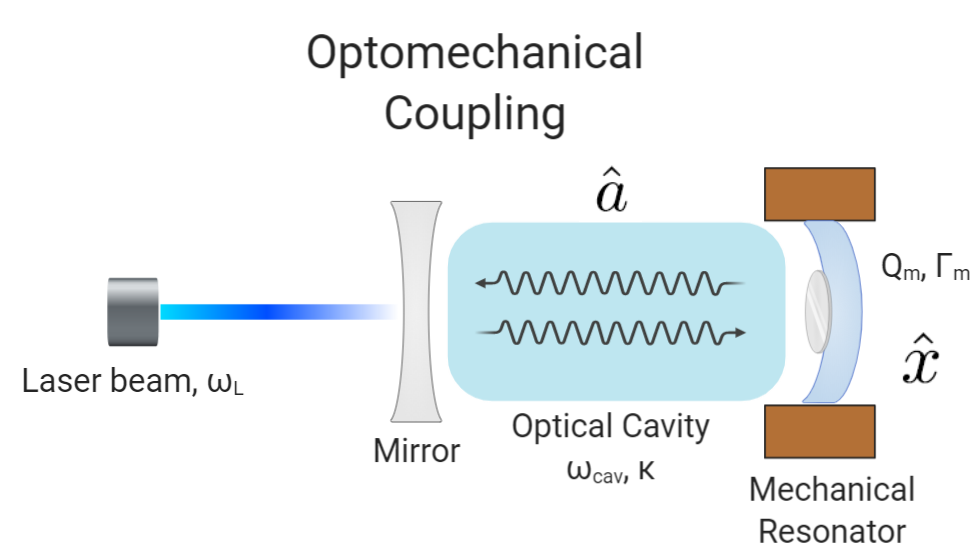
\includegraphics [width=\columnwidth, height=5cm] {Optomechanical_diagram.PNG}
    \caption{Illustration of optomechanical coupling between an optical cavity and a mechanical resonator. $\hat{a}$ denotes the photon annihilation operator. }
    \label{fig:Optomechanical_diagram}
\end{figure}

\subsubsection{Hamiltonian Formulation}

The uncoupled optical ($\omega_{cav}$) and mechanical ($\Omega_m$) modes are represented by two harmonic oscillators:

\begin{equation*}
    \hat{H}_o = \hbar \omega_{cav} \hat{a}^\dagger \hat{a} + \hbar \Omega_m \hat{b}^\dagger \hat{b}
\end{equation*}

In the case of a cavity with a movable end mirror, the frequency $\omega_{cav}$ is modulated by the mechanical amplitude:

\begin{equation*}
    \omega_{cav}(x) \approx \omega_{cav}  + x\frac{\partial \omega_{cav}}{\partial x} + \cdots
\end{equation*}

For most experimental realizations it suffices to keep the linear term, where we define the optical coupling per shift displacement as $ G = -\frac{\partial \omega_{cav}}{\partial x} $. For a simple cavity of length $L$, we have $G = \omega_{cav}/L$.
\newline

In general, expanding to the leading order in the displacement, we have:

\begin{equation*}
    \hbar \omega_{cav}(x) \hat{a}^\dagger \hat{a} \approx \hbar (\omega_{cav} - G \hat{x}) \hat{a}^\dagger \hat{a} 
\end{equation*}

Here $\hat{x} = x_{zpf}(\hat{b}^\dagger + \hat{b}) $ as defined before. Thus, the interaction part of the Hamiltonian can be written as:

\begin{equation*}
    \hat{H}_{int} = -\hbar g_o \hat{a}^\dagger \hat{a} (\hat{b}^\dagger + \hat{b} )
\end{equation*}

where $ g_o = G x_{zpf} $ is the vacuum optomechanical coupling strength, expressed as a frequency. It quantifies the interaction between a single phonon and a single photon.
\newline

The radiation pressure force is simply the derivative of $\hat{H}_{int}$ with respect to displacement:

\begin{equation*}
    \hat{F} = -\frac{d\hat{H}_{int}}{d\hat{x}} = \hbar G \hat{a}^\dagger \hat{a} =    \frac{\hbar g_o  \hat{a}^\dagger \hat{a} }{x_{zpf}}
\end{equation*}

Where $g = g_o \sqrt{\bar{n}_{cav}}$ is often referred to as the "optomechanical coupling strength". Note that the regime where $g > \kappa$ is known as the "strong-coupling" regime of cavity optomechanics, and when $\kappa << \Omega_m$ the system is in the sideband-resolved regime. Note that a practical threshold for room-temperature optomechanics is given as \cite{project_paper, cavity_optomechanics_2014}:

\begin{equation*}
    Q_m f_m >> k_B T / 2\pi \hbar = 6.25 \ THz
\end{equation*}

This requirement stems directly from Equation \ref{eq:coherent_oscillations}. Thus, any mechanical oscillator to be used in room-temperature optomechanics must satisfy this requirement.

\subsubsection{Types of Optomechanical Resonators}

There are many different types of optomechanical resonators which exist, each having their own merits for different applications. Some examples of these resonators are shown in Figures \ref{fig:optomechanical_resonators} and \ref{fig:optomechanical_devices}. Specific designs are shown in Appendix \ref{Types of optomechanical resonators}. We discuss some specific parameters of a few designs in Section \ref{Thoughts}.

\begin{figure}[htb]
    \centering
    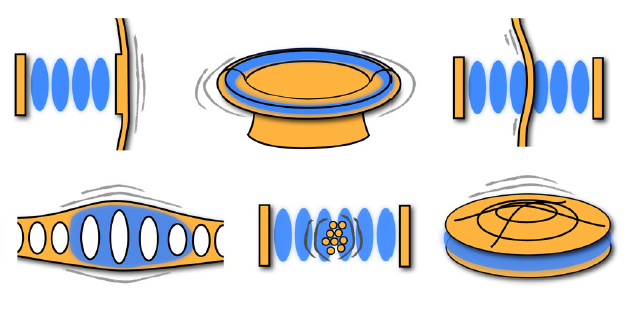
\includegraphics[width=\columnwidth, height=5cm]{optomechanical_resonators.PNG}
    \caption{From \cite{cavity_optomechanics_2014}: \textit{"Common optomechanical resonators with their respective mode shapes and vibrational degrees of freedom shown. From left to right, and top to bottom: a suspended mirror, a microtoroid, a nano-object (or a membrane) inside an optical cavity, localized modes in a photonic crystal nanobeam, a trapped and vibrating cold atom cloud (or other levitated object) inside a cavity, and a vibrating drum
    capacitor coupled to a microwave field."}}
    \label{fig:optomechanical_resonators}
\end{figure}


\section{Strain Engineering}\label{Strain Engineering}

Materials can be subject to stresses up to a certain threshold before they are subject to inelastic relaxation; this threshold is given by their yield stress $\sigma_y$. Up to this limit, any force applied to the system will result in a strain in the system, which is an elongation of the material per unit length, or $\epsilon = \Delta L / L_0 = (L-L_0)/L_0$, where $L$ is the length after applying a stress, and $L_0$ is the initial length. For stresses $\sigma$ up to $\sigma_y$, we expect the strain response to behave in a linear/elastic manner, such that $\sigma = E \epsilon$, where $E$ is the Young's modulus for the material. In this regime, if the material is allowed to relax after being strained, it will return to its original unperturbed length $L_0$. Outside of this regime, there is a nonlinear dependence of $\epsilon$ on $\sigma$, such that inelastic/plastic relaxation occurs when the material is allowed to relax after being strained. The stress-strain curve for silicon nitride is shown in Figure \ref{fig:stress_strain_Si3N4}. One can also define a quantity known as Poisson's ratio, which characterizes the deformation of the material, and is given by $-\frac{\epsilon_l}{\epsilon_t}$, which is the negative of the ratio of the longitudinal strain to the tangential strain.
\newline

To quote \cite{elastic_strain_engineering} for a broad understanding of the phenomenon of elastic strain engineering:
\newline

\textit{"Nanostructured materials such as thin films, nanowires, nanoparticles,
bulk nanocomposites, and atomic sheets can withstand non-hydrostatic (e.g., tensile or shear) stresses up to a significant fraction of their ideal strength without inelastic relaxation by plasticity or fracture. Large elastic strains, up to $\sim 10\%$, can be generated by epitaxy or by external loading on small-volume or bulk-scale nanomaterials and can be spatially homogeneous or inhomogeneous. This leads to new possibilities for tuning the physical and chemical properties of a material, such as electronic, optical, magnetic, phononic, and catalytic properties, by varying the six-dimensional elastic strain as continuous variables. By controlling the elastic strain field statically or dynamically, a much larger parameter space opens up for optimizing the functional properties of materials, which gives new meaning to Richard Feynman’s 1959 statement, “there’s plenty of room at the bottom.”}
\newline

Therefore the mechanical properties of a resonator can be enhanced, for instance, by applying the principles of elastic strain engineering. Therefore, the enhancement of the $Qf$ product of a nanobeam resonator is achived by Ghadimi et al. \cite{ghadimi_main_paper} by locally enhancing the strain in the nanobeam. This is discussed in the following section. 

\begin{figure}[H]
    \centering
    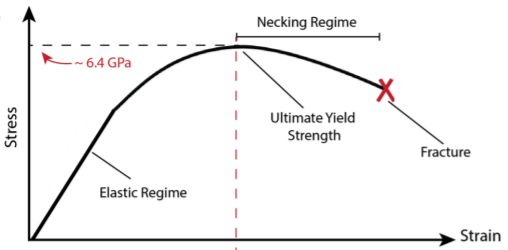
\includegraphics[width = \columnwidth]{stress_strain_Si3N4.PNG}
    \caption{Stress-strain characteristics for $Si_{3} N_{4}$ \cite{mechanical_resonators_optomechanics_room_temp}}
    \label{fig:stress_strain_Si3N4}
\end{figure}


\subsection{Dissipation Dilution and Soft Clamping}\label{Dissipation Dilution and Soft Clamping}
In this section we present the results obtained by Ghadimi et al. \cite{generalized_dissipation_dilution} for generalized dissipation dilution in strained mechanical resonators. In particular, we see how this theory applies to the particular geometry of interest as discussed in Section \ref{COMSOL results}. We refer the interested reader to go through the derivation of these in \cite{generalized_dissipation_dilution, ghadimi_main_paper}. 
\newline

The dissipation of mechanical motion is in general a complicated phenomenon at the nanoscale, involving both intrinsic and surface loss mechanisms and is yet to be well understood. Dissipation mechanisms lead to decoherence of quantum states, as well as introduces noise, which severely limits the ability to detect forces with precision. Therefore, it is of interest to limit these dissipative loss mechanisms to achieve higher quality factor mechanical resonators.
\newline

The quality factor $Q$ of a mechanical oscillator generally does not exceed the inverse of the material loss angle, $\phi$, characterizing the delay between the stress and strain in the material (see Equation \ref{stress-strain-relation}). However, through dissipation dilution $Q$-factors much larger than $1/\phi$ can be achieved. Note that it is mentioned in \cite{generalized_dissipation_dilution} that the cause of dissipation dilution arising in a resonator are still unclear, other than the mere presence of tensile strain. It is also unclear whether any modes other than the flexural mode experience dissipation dilution. 
\newline

The intrinsic value of the resonator quality factor is given by $Q_{int} = 1/\phi$. If $\omega_{dil}$ is the natural frequency of motion in a lossless potential, then the quality factor is increased by the "dilution factor" \footnote{The diluted quality factor $Q$ can also be interpreted as the ratio of the real and imaginary parts of the eigenfrequency of the resonator \cite{ghadimi_thesis}}:

\begin{equation}\label{D_Q}
    D_Q = \frac{Q}{Q_{int}} = \frac{\omega_{int}^2 + \omega_{dil}^2}{\omega_{int}^2}
\end{equation}  

We can write the strain tensor with respect to the total deformation field $\Tilde{U}_{i}(x, y, z, t) (i = x, y, z)$ as:

\begin{equation}\label{strain tensor}
    \Tilde{e}_{ij} = \frac{1}{2} \Big ( \frac{\partial \Tilde{U}_i}{\partial x_j} + \frac{\partial \Tilde{U}_j}{\partial x_i} + \frac{\partial \Tilde{U}_l}{\partial x_i}\frac{\partial \Tilde{U}_l}{\partial x_j} \Big )
\end{equation}

Where summation over repeating indices is implied. The last term in the equation above is nonlinear in displacement this is what we call geometric nonlinearity. The strain tensor can be split into static $e_{ij}$ and time-dependent $\Delta e_{ij}(t)$ contributions:

$$ \Tilde{e}_{ij}(t) = e_{ij} + \Delta e_{ij}(t) $$

In the simplified case where the stress-strain relation omits Poisson's ratio (ratio of the lateral strain to the tensile strain), $\nu$, the relation is given as:

\begin{equation}\label{stress-strain-relation}
     \Tilde{\sigma}_{ij}[w] = E e^{-i\phi} \Tilde{e}_{ij}[w] 
\end{equation}

The dilution factor can be rewritten from Equation \ref{D_Q} as:

\begin{equation}
    D_Q = 1 + \frac{\int 2e_{ij} \big \langle \Delta e_{ij}(t) \big \rangle dV}{\int \big \langle \Delta e_{ij}(t)\Delta e_{ij}(t) \big \rangle dV}
\end{equation}

Note that if the static strain $e_{ij}$ is zero, then $D_Q = 1$, corresponding to no $Q$-enhancement. $D_Q$ can also be less than or greater than unity if $e_{ij} \neq 0$ and $\Delta e_{ij}(t) \neq 0$, with the latter being possible only if there is geometric nonlinearity in the structure (i.e. the nonlinear term in Equation \ref{strain tensor} is nonzero). 
\newline

The lossless potential generalizing tension energy can thus be expressed as:

\begin{equation*}
    \Big \langle W_{dil}(t) \Big \rangle \equiv E \int e_{ij} \Big \langle \Delta e_{ij}(t) \Big \rangle dV
\end{equation*}

This corresponds to $\omega_{dil}$ in Equation \ref{D_Q}. The lossy part of the energy which generalizes the bending energy can be expressed as:

\begin{equation*}
    \Big \langle W_{lossy}(t) \Big \rangle \equiv \frac{E}{2} \int\Big \langle \Delta e_{ij}(t) \Delta e_{ij}(t) \Big \rangle dV
\end{equation*}

This corresponds to $\omega_{int}$ in Equation \ref{D_Q}. We can then see that a combination of tension and a large geometric nonlinear contribution to the dynamic strain leads to strong dissipation dilution.
\newline

For beam geometries, $D_Q$ may be written as:

\begin{equation*}
    D_Q = 1 + \frac{\int 2\epsilon \big \langle \Delta \epsilon(t) \big \rangle dV}{\int \big \langle \Delta \epsilon(t)^2 \big \rangle dV}
\end{equation*}

For flexural modes of a uniform rectangular beam with mode number n, $D_Q$ can be expressed as:

\begin{equation*}
    D_{Q,n} = \frac{1}{2\lambda + \pi^2 n^2 \lambda^2}
\end{equation*}

Where $\lambda$ is defined as:

\begin{equation*}
    \lambda^2 = \frac{h^2}{12 l^2 \epsilon_{avg} }
\end{equation*}

Where $h$ is the thickness, $l$ is the beam length, and $\epsilon_{avg}$ is the volume-averaged static tensile strain in the beam.

For a general beam, the dissipation dilution factors are given as:

\begin{equation*}
    D_{Q,n} = \frac{1}{2\alpha_n \lambda + \beta_n \Omega_n^2 \lambda^2}
\end{equation*}

Where $\Omega_n$ is the dimensionless frequency of the n-th mode:

\begin{equation*}
    \Omega_n^2 = \frac{\rho l^2 \omega_n^2}{\epsilon_{avg} E}
\end{equation*}

The beam shape-dependent clamping and distributed loss coefficients $\alpha_n$ and $\beta_n$ are given as:

\begin{equation*}
    \alpha_n = \frac{\sqrt{v_{cl}} (u^{'}_{cl,n})^2}{2\Omega_n^2 \big ( \int_{0}^{1} v(s) u_n(s)^2 \big ) ds}
\end{equation*}

\begin{equation*}
    \beta_n = \frac{\int_{0}^{1} v(s)^3 u_{n}(s)^2 ds}{\int_{0}^{1} v(s) u_{n}(s)^2 ds}
\end{equation*}

Here, $(u^{'}_{cl,n})$ is the spatial derivative of the mode shape computed near the clamping points, $u_n(s)$ is the mode shape, $s = x/l$ is the scaled coordinate along the beam, and $v(s) = w(s)/\omega_{avg}$ is the beam width variation normalized with respect to the average beam width. One can then think of dissipation dilution of a non-uniform beam entirely in terms of the reduction of $\alpha_n$, $\beta_n$ by varying the beam width $w(x)$. 
\newline

For the transverse mode, the strain and width are related as follows:

\begin{equation*}
    \frac{\epsilon(x)}{\epsilon_{avg}} = \frac{w_{avg}}{w(x)}
\end{equation*}

Using this relation and assuming that the clamping loss coefficient is negligible ($\alpha_n \approx 0$), in addition to setting an upper bound on the strain as given by the yield strain $\epsilon_{yield}$, we obtain:

\begin{equation*}
    \beta_n \geq \Big ( \frac{\epsilon_{avg}}{\epsilon_{yield}} \Big ) ^2
\end{equation*}

Which leads to an upper bound for the dilution factor:

\begin{equation*}
    D_Q \leq \frac{12 E \epsilon^{2}_{yield}}{\rho h^2 \omega^2}
\end{equation*}

We now consider dilution factors for different beam designs. In \cite{generalized_dissipation_dilution}, there are three main designs discussed, namely phononic crystal (PnC) beams, thin clamps, and tapered PnC beams. 

\subsubsection{Soft Clamping}
To quote \cite{generalized_dissipation_dilution}:
"Soft clamping refers to the suppression of clamping losses by localizing a flexural mode in a phononic crystal. A one-dimensional PnC can be formed by periodically modulating the beam width. " The dilution factors for soft-clamped beams are given by:

\begin{equation*}
    D_Q = \frac{12E {\epsilon}_{film}^2}{(1-\nu)^2 \rho h^2 \omega^2}
\end{equation*}

The localized modes of the PnC beam approach the performance of ideal clamp-less beams. The clamping loss coefficient can be estimated as:

\begin{equation*}
    \alpha_n = e^{(1-n)/n_L}
\end{equation*}

Where $n_L$ is the mode amplitude decay length in units of acoustic half-wavelengths. The optimization of $D_Q$ with respect to $n$ leads to the following expression:

\begin{equation*}
    \frac{1}{\pi^2 n^{2}_{max} \lambda^2}
\end{equation*}

Where $n_{max}$ (typically $>>1$) is the optimum localized mode order. Since $n_{max}>>1$, we require $\lambda<<1$ for a high $D_Q$ factor. This implies that $l>>h$, or that the beam has a high aspect ratio.

\subsubsection{Thin Clamping}
Thin clamping involves reducing the beam width near the clamping regions, $v_{cl} = w(0)/w_{avg}$. Since $\alpha_n \propto \sqrt{v_{cl}}$, it can be reduced by making the clamps thinner. Physically, this corresponds to enhancing the strain in the clamping regions. $\lambda$ is then reduced to:

\begin{equation*}
    \lambda_{cl} = \sqrt{h^2 / 12 \epsilon_{cl} l^2}
\end{equation*}

Where $\epsilon_{cl} = \epsilon_{avg}/v_{cl}$ is the local strain. Then $D_Q$ is given as:

\begin{equation*}
    D_{Q,n} \approx \frac{1}{2\lambda_{cl} + (n\pi)^2 \lambda^2}
\end{equation*}

Thin-clamped beams have improved $D_Q$ factors over soft clamping for lower-order vibrational modes.

\subsubsection{Tapered PnC Beams}\label{PnC}
In contrast to both soft clamping and thin clamping, tapered PnC beams also offer reduction of the distributed loss coefficient $\beta_n$. This is achieved by co-localizing the flexural mode and region of enhanced strain away from the clamps. The width of the PnC beam is tapered as \cite{generalized_dissipation_dilution, ghadimi_main_paper}:

\begin{equation}\label{width tapering}
    w_{cell,i} \propto 1 - (1-\alpha_w) exp(-i^2/i_{o}^2)
\end{equation}

Where $i = 0, 1, \cdots$ is the cell index starting from the center unit cell, and $a_w, i_o$ define the transverse and longitudinal sizes of the waist region, respectively \footnote{Here $a_w, i_o$ were optimized using a random search algorithm by Ghadimi et al. in \cite{generalized_dissipation_dilution}, with $a_w = 0.15-0.2$, and $i_o = 8-10$}. The PnC cell lengths are also scaled as $1/\sqrt{w_{cell}}$ to compensate for the bandgap frequency shift due to the non-uniform strain distribution \cite{generalized_dissipation_dilution}. Assuming that the mode is localized in the waist region with width $v_{waist}$ and that clamping losses are negligible, the dilution factor is given by:

\begin{equation*}
    D_{Q,n} \approx \frac{1}{\Omega_{waist}^2 \lambda_{waist}^2 }
\end{equation*}

Where:

\begin{equation*}
    \Omega_{waist}^2 = \rho l^2 w^2 / (\epsilon_{waist} E)
\end{equation*}
\begin{equation*}
    \lambda_{waist}^2 = h^2 / (12 \epsilon_{waist} l^2)
\end{equation*}

With $\epsilon_{waist} = \epsilon_{avg} / v_{waist}$. In the limit that $v_{waist}$ approached the yield value, the ultimate limit of dissipation dilution can be achieved. To quote \cite{generalized_dissipation_dilution}: " A practical limitation for dissipation dilution enhancement by strain concentration in this case originates from the tradeoff between $\epsilon_{waist}$ and the waist length. Substantially increased strain is only achievable over a small fraction of the beam length, therefore only short-wavelength and high-frequency modes can benefit from such global geometric strain engineering.".


\subsubsection{Summary}
Thus it was seen that a lossless contribution to the elastic energy (which gives rise to Q-enhancement via dissipation dilution) arises as a presence of static strain and geometric nonlinearity in the material. High aspect ratio beams can produce high dissipation dilution, as was seen above. The reason for dissipation dilution may be interpreted entirely in terms of the minimization of the loss coefficients $\alpha_n$ and $\beta_n$.
\newline


The various beam geometries addressed above can be represented graphically in Figure \ref{fig:D_Q various beam designs} (from \cite{generalized_dissipation_dilution}. We can see here that the tapered PnC design is superior to the other designs in terms of the $Qf$ product.

\begin{figure}
    \centering
    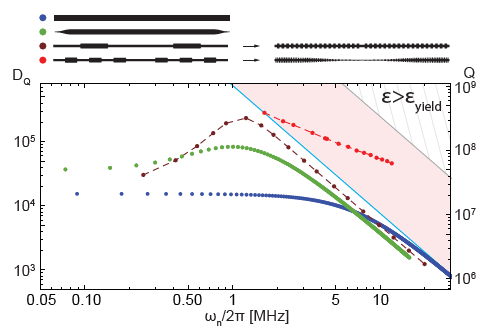
\includegraphics[width=\columnwidth]{D_Q_various_beam_designs.PNG}
    \caption{From \cite{generalized_dissipation_dilution}: \textit{"Dissipation dilution in beams with different transverse profiles, assuming a fixed length $l = 3 \ mm$ and thickness $h = 20 \ nm$. Points correspond to $D_Q$ (left axis) and $Q$ (right axis) for special flexural modes, assuming $Qint = 1.4 \cdot 10^3$. Blue and green points correspond to modes of uniform and thin-clamped ($v_{cl} = 0.14$) beams. Dark red and red points correspond to localized modes of PnC beams and tapered PnC beams, respectively. Note that each localized mode corresponds to a different beam profile. Blue line: ideal limit for a soft-clamped beam. Gray line: ideal limit for a clamp-free beam strained to the yield point."}}
    \label{fig:D_Q various beam designs}
\end{figure}


Assuming that the resonator dissipation is due to intrinsic losses, the following relation can be asserted \cite{generalized_dissipation_dilution}:

\begin{equation*}
    Q = D_Q \times Q_{int}
\end{equation*}

Where $Q_{int}$ is the intrinsic quality factor of the beam. For $Si_3 N_4$ beams with thickness less than $100 \ nm$, it was shown in \cite{ generalized_dissipation_dilution} (Supplementary Materials) that the intrinsic quality factor is a function of its thickness:

\begin{equation}\label{Q_int(h)}
     Q_{int}(h) = 6900 \frac{h}{[100 \ nm]}
\end{equation}



% \section{Loss Mechanisms in Nanomechanical Resonators} % Now in Section II


\section{COMSOL Simulation Results}\label{COMSOL results}
Here we present the simulations done in COMSOL Multiphysics for the motion of a $Si_{3}N_{4}$ tapered PnC (i.e. nanobeam). The nanobeam was analyzed using the Solid Mechanics module in COMSOL. 
\newline

The nanobeam design considered was the tapered PnC nanobeam as considered in Section \ref{PnC} due to their superior $Qf$ product, which is what we desire for an optomechanical transducer. For the specific design of the nanobeam, the work of Ghadimi et al. \cite{generalized_dissipation_dilution, ghadimi_main_paper} was followed \footnote{The program used to generate the nanobeam parameters is available at \cite{ruchir_nanobeam_program}}. The widths of the unit cells were thus tapered according to Equation \ref{width tapering}. The unit cell lengths were tapered according to:

\begin{equation*}
    L_{c}(i) \propto 1 / \sqrt{w_{max}(i)}
\end{equation*}

Where $w_{max}(i)$ denotes the $i^{th}$ unit cell maximum width. Figure \ref{fig:unitcell_design} illustrates the tapering of the unit cell widths and lengths for the tapered PnC nanobeam design.

\begin{figure}[H]
    \centering
    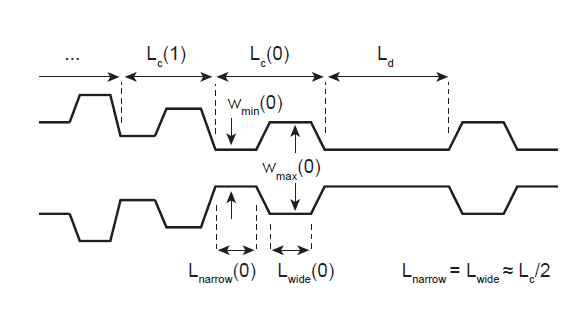
\includegraphics[width = \columnwidth]{unitcell_design.PNG}
    \caption{Nanobeam design \cite{generalized_dissipation_dilution} (Supplementary Materials)}
    \label{fig:unitcell_design}
\end{figure}

The procedure to build the geometry in COMSOL was as such: given the width and length parameters of the nanobeam, the geometry as per Figure \ref{fig:unitcell_design} was constructed using simple rectangles to represent the minimum and maximum width areas of the unit cells. This was done in 2D, and was then extracted to 3D using the height parameter. 

\begin{figure}[H]
    \centering
    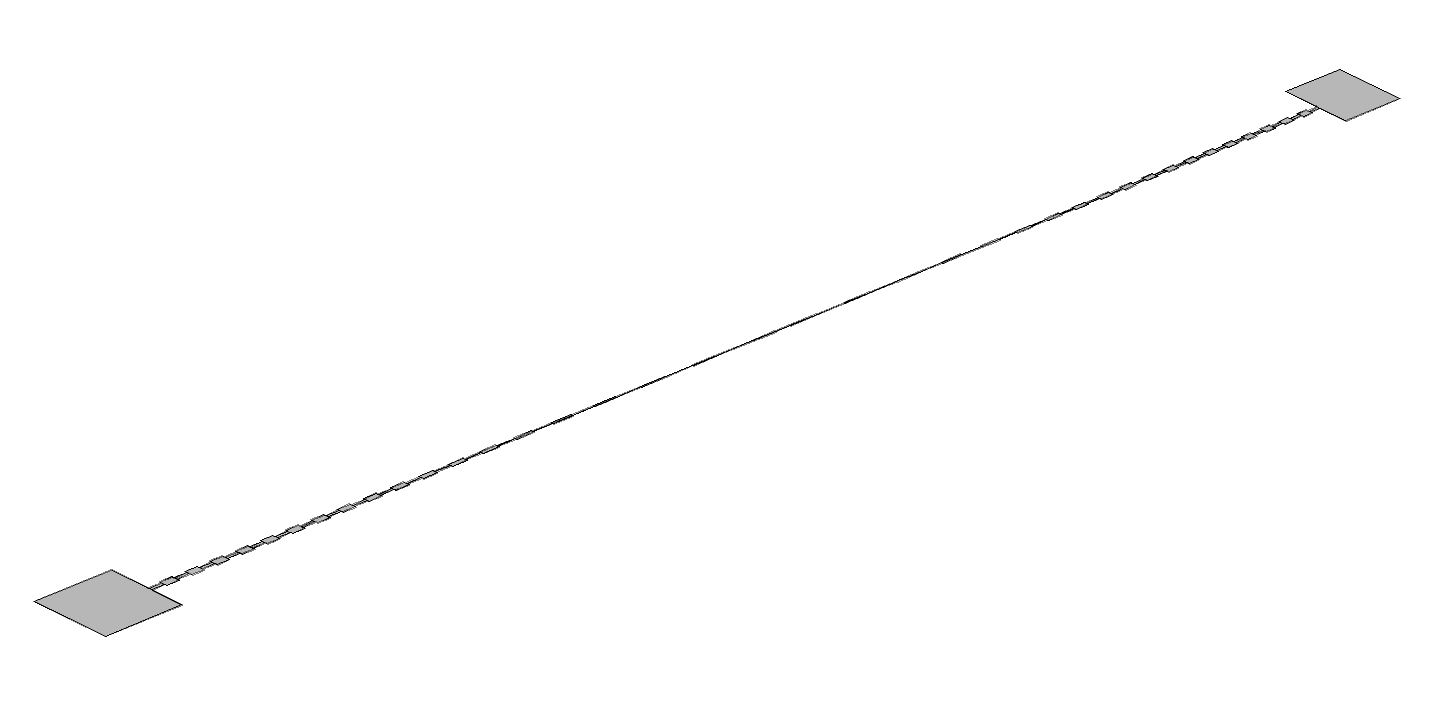
\includegraphics[width = \columnwidth]{COMSOL_nanobeam_geometry.png}
    \caption{3D view of nanobeam geometry in COMSOL. Note that the larger blocks at the end are the supports used to clamp the nanobeam at the ends. Here, the tapering is not so obvious due to the large aspect ratios. Parameters used: beam length = $4 \ mm$, height = $20 \ nm$, minimum beam width = $400 \ nm$, central defect length = $50 \ \mu m$, 38 unit cells.}
    \label{fig:COMSOL_nanobeam}
\end{figure}

The mesh selected for the study was an "extremely fine" user-controlled mesh. This was done so that the edges of the geometry are effectively resolved into mesh polygons. Refer to Appendix \ref{FEM_method_Strauss} for more details on the Finite Element Method, which is the numerical method used by COMSOL to solve for the relevant equations over the geometry, which in this case is the entire nanobeam. Here we present the two cases of meshing as seen in COMSOL (Figures \ref{fig:nanobeam_mesh_supports}, \ref{fig:nanobeam_inner_mesh}); the meshing algorithm resolves the end supports and inner regions of the unit cells differently, but with no loss of generality in terms of the solutions:

\begin{figure}[H]
    \centering
    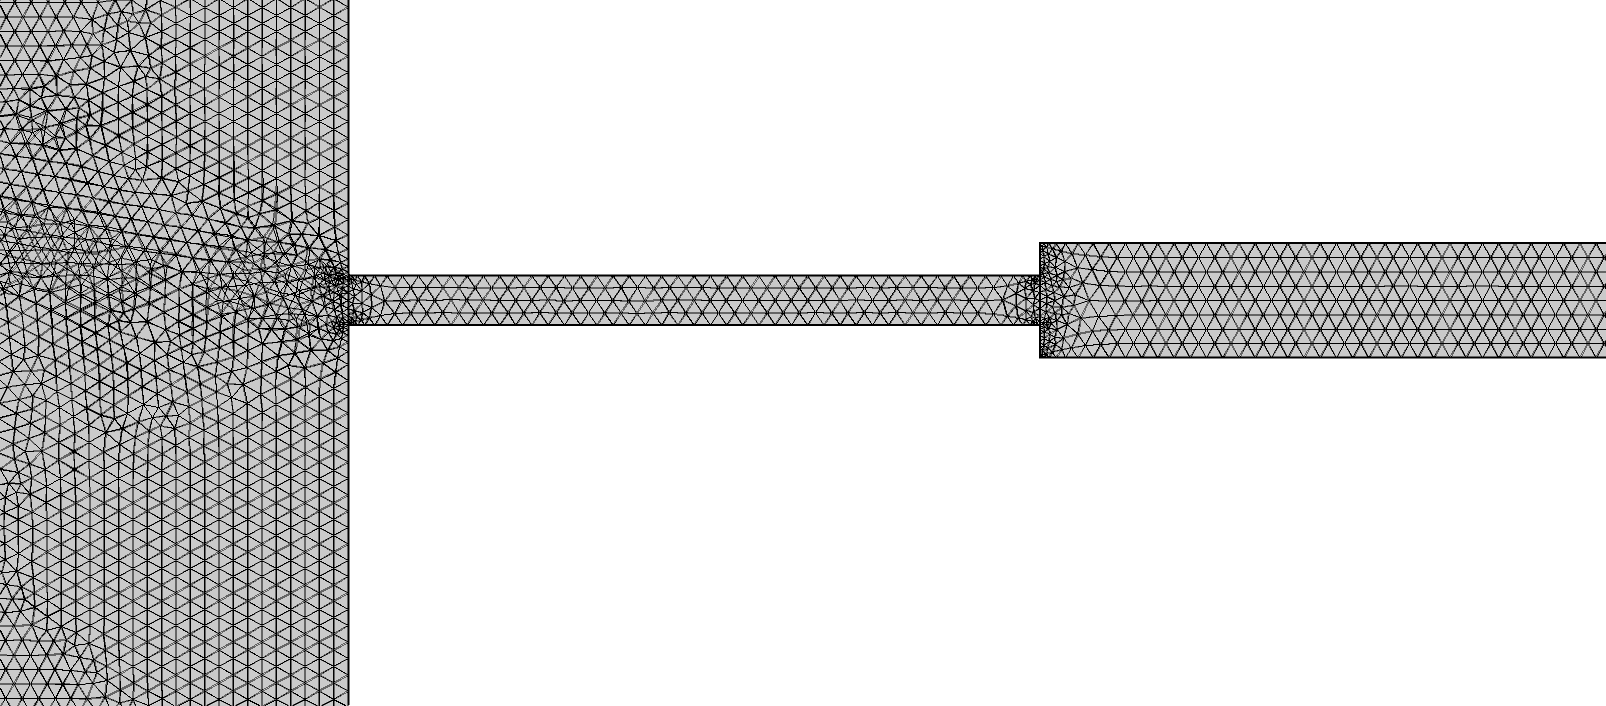
\includegraphics[width = \columnwidth]{nanobeam_mesh_supports.png}
    \caption{Nanobeam meshing near supports}
    \label{fig:nanobeam_mesh_supports}
\end{figure}

\begin{figure}[H]
    \centering
    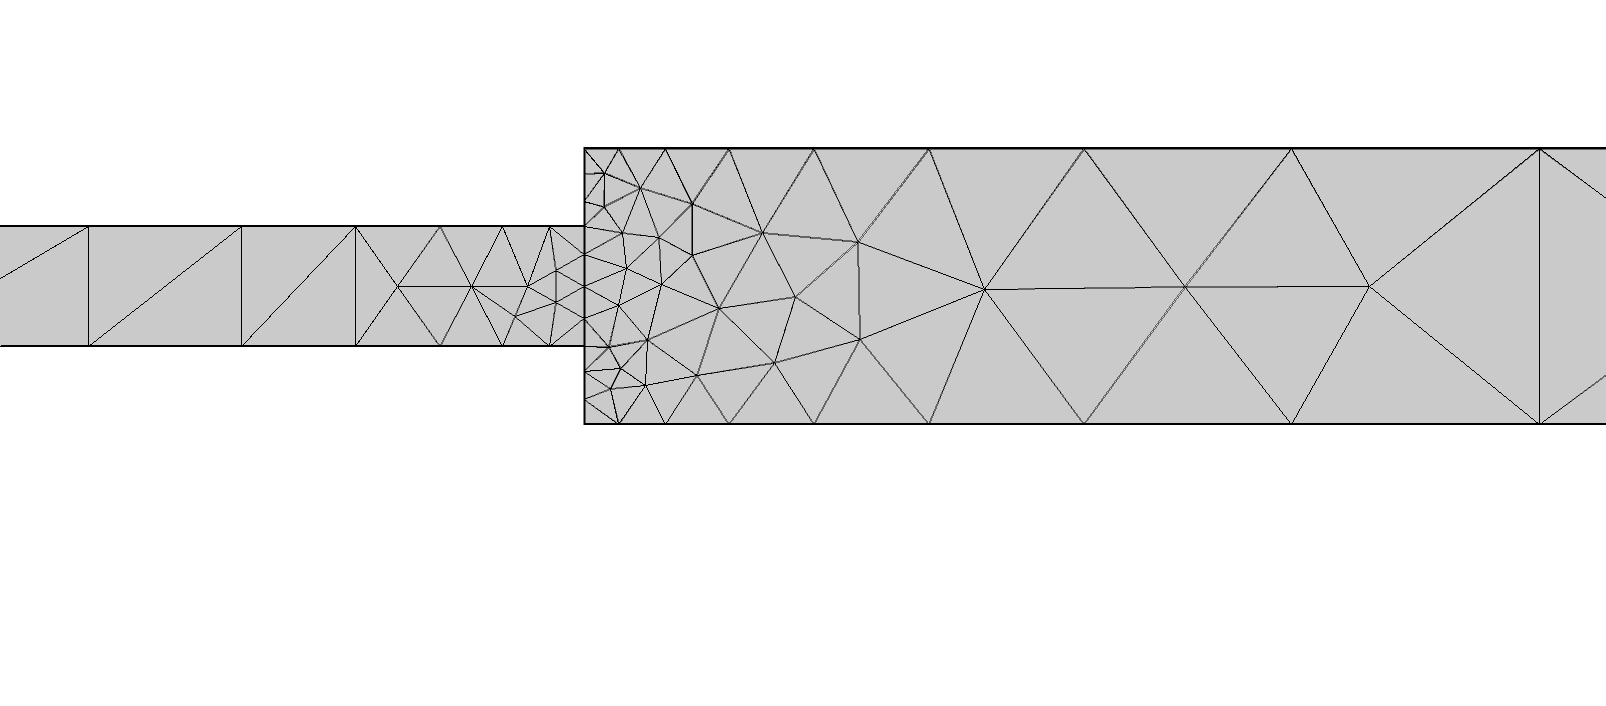
\includegraphics[width = \columnwidth]{nanobeam_inner_mesh.png}
    \caption{Nanobeam meshing along inner unit cells}
    \label{fig:nanobeam_inner_mesh}
\end{figure}

The mode shape was analyzed by performing an eigenfrequency analysis on the nanobeam after applying a uniform distributed load of $10^{-9} \ N/m^3$. The decision to apply a distributed load instead of a point load is justified by the fact that the radiation pressure acts all along the nanobeam, thus oscillations of the nanobeam are due to the resultant force caused by this. The value of the distributed load is somewhat arbitrary, a nanoscale force seems like a reasonable choice considering the mass of the nanobeam considered is on the order of picograms \cite{ghadimi_main_paper}. An eigenfrequency search \footnote{There is an option in COMSOL at the \textit{Study} node listed as "Include geometric nonlinearity". This was selected, and according to \cite{what_is_geometric_nonlinearity}, has the same effect as described in section \ref{Dissipation Dilution and Soft Clamping}.} was conducted, and 100 eigenfrequencies were computed around $0 \ Hz$. The mode shape with the closest behaviour to the results in \cite{ghadimi_main_paper} observed for the parameters described in Figure \ref{fig:COMSOL_nanobeam} is shown in Figure \ref{fig:Nanobeam_mode_shape_35194Hz}:

\begin{figure}[H]\label{Mode Shape}
    \centering
    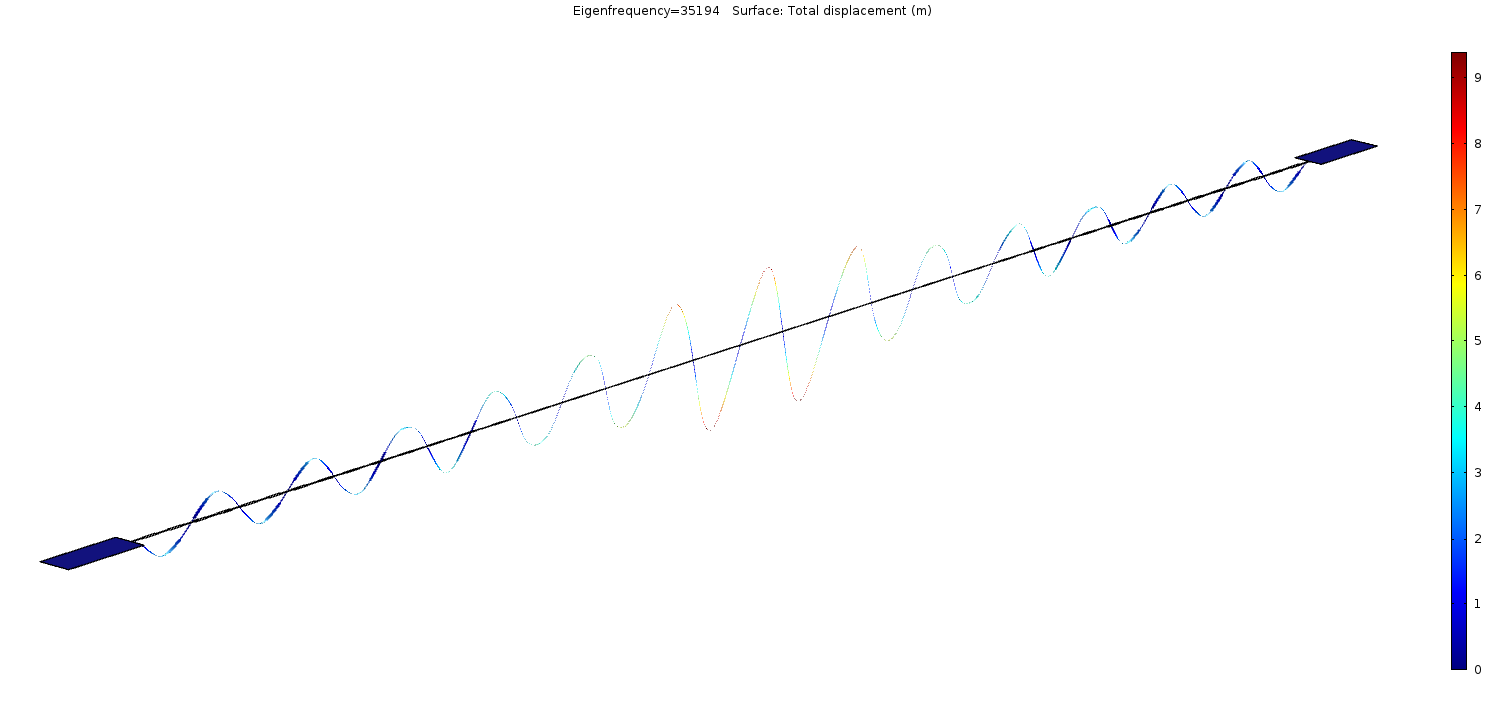
\includegraphics[width = \columnwidth]{Nanobeam_mode_shape_35194Hz.png}
    \caption{Mode shape for nanobeam oscillating at 35194 Hz in the transverse mode. We can see that there is a much larger displacement near the central defect than near the clamps, which is what we expect to see.}
    \label{fig:Nanobeam_mode_shape_35194Hz}
\end{figure}

Here we can see that the mode shape is localized around the central defect. However, the effect is not as pronounced as in \cite{ghadimi_main_paper}, which suggests that more work needs to be done yet to refine the simulation. The eigenfrequency is on the order of $10^4 \ Hz$ (Figure \ref{Mode Shape}). The mode shape is not as pronounced as the mode shape shown by Ghadimi et al. \cite{ghadimi_main_paper}.  Some reasons for this are discussed in Section \ref{Conclusion}. Larger PnC beams (i.e. more unit cells) may potentially lead to more localized mode shapes.  

% Using Equations \ref{D_Q} and \ref{Q_int(h)} with $h = 20 \ nm$, we get that the $Q$ factor for the beam is $48,576,720 \sim 5 \cdot 10^7$. This is not very close to the value of $10^9$ obtained by Ghadimi et al. \cite{ghadimi_main_paper}. 

% Some reasons for this are discussed in Section \ref{Conclusion}. Larger PnC beams (i.e. more unit cells) may potentially lead to higher observed $Q$ factors.

\section{Thoughts on other potential resonator designs}\label{Thoughts}

To achieve a good spin-photon interface as described in \cite{project_paper}, we require high $Qf$ products. While the results achieved by Ghadimi et al. are the highest till date ($Qf \sim 10^{15} \ Hz$ for an effective mass of $\sim pg$ \cite{ghadimi_main_paper}), other resonator designs may also provide suitable characteristics for the interface. Examples of such designs can be seen in Figures \ref{fig:optomechanical_resonators}, \ref{fig:optomechanical_devices}. A lower effective mass is preferred as described in \cite{project_paper} due to the relaxation of the magnitude of the magnetic field gradient.
\newline

Trampoline membranes were considered in \cite{project_paper} as a potential mechanical resonator used in the transducer system. However, these are relatively large structures, having larger characteristic masses ($\sim 10^2 \ ng$) compared to nanobeams. In addition, these have quality factors typically on the order of $10^7$, and frequencies on the order of $10^5 \ Hz$, resulting in a $Qf$ product of $\sim 10^{12} \ Hz$ \cite{mechanical_resonators_optomechanics_room_temp, SiN_trampoline_resonators}. Thus, in terms of both effective mass and $Qf$, they are inferior to the tapered PnC nanobeam design. 
\newline

Carbon nanotubes (CNTs) are also a potential resonator design to be considered. These typically have quality factors on the order of $10^3$, and frequencies on the order of $10^5 \ Hz$, resulting in a $Qf$ product of $\sim 10^8 \ Hz$. However, CNTs have very small effective masses, on the order of $10^{-18} \ kg$ \cite{CNT_resonator}, which may be beneficial for some applications. The transducer system proposed in \cite{project_paper} requires a magnetic field for the coupling of the NV center to the mechanical oscillator; this is typically done by adding a magnetic tip to the end of the mechanical oscillator. We present a calculation to instead generate a magnetic field by passing a current through a carbon nanotube in Appendix \ref{Current Calculations}, and show that it is not advisable to use this method to generate a magnetic field to couple to an NV center. Hence, CNTs are inferior to the tapered PnC nanobeam design in terms of $Qf$ product, however they are superior in terms of effective mass. 
\newline

Other designs are possible, as can be seen in Figures \ref{fig:optomechanical_resonators}, \ref{fig:optomechanical_devices}, however these were not explored in much detail. Figure 10 of \cite{cavity_optomechanics_2014}, shown above, shows the $Q(f)$ for various published experiments.

\begin{figure}
    \centering
    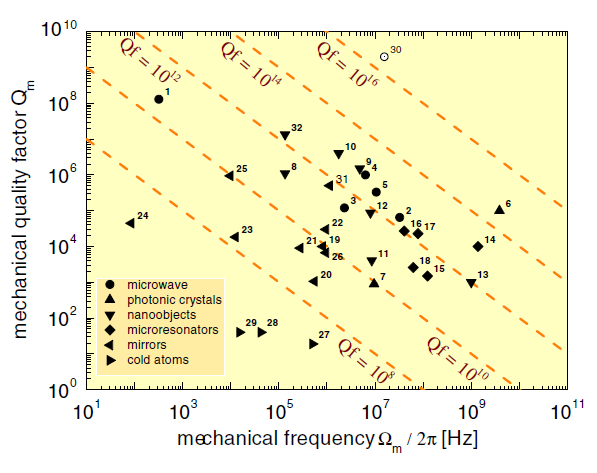
\includegraphics[width = \columnwidth]{Qf_other_designs.PNG}
    \caption{From \cite{cavity_optomechanics_2014}: \textit{"Mechanical quality factor $Q_m = \Omega_m / \Gamma_m$ vs mechanical frequency $\Omega_m = 2\pi f_m$ for published experiments $\cdots$ The dashed lines represent constant $Q_m f_m$ values."} See \cite{cavity_optomechanics_2014} for the experiments corresponding to the numbers.}
    \label{fig:Qf_other_designs}
\end{figure}


\section{Conclusions and Outlook}\label{Conclusion}
In this report we have looked at some of the theory of optomechanics and strain engineering. We then saw its application in COMSOL Multiphysics to a tapered PnC nanobeam. We saw that dissipation dilution arose as a result of geometric nonlinearity and static strain in the beam, and by tuning the shape and strain of the nanobeam one can achieve higher $Q$ factors.
\newline

While the results obtained in Section \ref{COMSOL results} do not exactly agree with the results obtained by Ghadimi et al. \cite{ghadimi_main_paper} in regards to the exact mode shape, the tapered PnC model can be further improved for the future. In particular, the approximation of the unit cell geometry as rectangles rather than the more complex shape in Figure \ref{fig:unitcell_design} may have led to the observed deviations from the expected result (possibly due to the bandgap frequency shift due to the geometric change). However, if this is corrected, then we would expect to see the correct result. However, we are hopeful that the tapered PnC geometry may lead to an improved quantum transducer system as described in \cite{project_paper} by providing a high $Qf$ product on the order of $10^{15}$ \cite{ghadimi_main_paper}.
\newline

In addition, the multiphysics coupling of a mechanical resonator to a Fabry-P\'erot cavity as well as a Nitrogen-Vacancy (NV) center is required to fully quantify the effects of the tapered PnC resonator to the transducer system in \cite{project_paper}. Both the Fabry-P\'erot cavity as well as the NV center models in COMSOL can be found at \cite{fabry_perot_cavity, NV_center_fluorescence}.

\subsection{Acknowledgements}
The author would like to acknowledge his supervisors Professor Christoph Simon and Stephen Wein for providing guidance and support during this project. In addition, the author would also like to thank Farid Ghobadi, Jiawei Ji, Yufeng Wu, Sourabh Kumar, Sumit Goswami, Hamidreza Kaviani and Bishnupada Behera for the assistance they provided as well as for the helpful discussions. The author would also like to thank the University of Calgary and the Institute for Quantum Science and Technology for the financial support provided. 

% The many discussions and team meetings were a critical aspect of the completion of this project as well as developing a good understanding of the concepts involved.

\newpage
% Begin appendix
\appendix

\section{COMSOL Multiphysics Simulations}


\subsection{Finite Element Method}\label{FEM_method_Strauss}
Given some domain $\Omega$ over which we want to compute some partial differential equation (PDE), we want to partition the domain into smaller, simpler polygons over the domain. This will allow for an approximation to the solution of the PDE by simpler functions on these partitioned sub-domains.
\newline

For example (taken from \cite{Strauss_PDES}), we consider the Dirichlet problem for Poisson's equation:

\begin{center}
$ -\Delta u = f $ in $\Omega$, where $u = 0$ on $\partial \Omega$ =  boundary of $\Omega$ 
\newline
\end{center}

We partition the domain into a finite sequence of simpler polygons (e.g., triangles as shown in \ref{fig:FEM}) with vertices $V_1, \dots ,V_n$. We pick trial functions $v_1(x,y), \dots , v_n(x,y)$ for each vertex such that these functions are equal to 1 at its vertex $V_i$ and zero at all other vertices. We approximate $u(x,y)$ by a linear combination of the trial functions:

\begin{equation}\label{eq:FEM1}
     u_N(x,y) = U_1 v_1(x,y) + \dots + U_N v_N(x,y)
\end{equation}


Where $U_1, \dots , U_n$ are coefficients. We can multiply Poisson's equation by any function $v(x,y)$ that vanishes on the boundary. Then:

\begin{equation}\label{eq:v_xy}
 \int\int_{\Omega} \nabla u \cdot \nabla v \ dx  \ dy = \int \int_{\Omega} f \ v  \ dx  \ dy 
\end{equation}


Requiring the above to be valid only for the first N special trial functions, $v_j = v_1, \dots ,v_n$. We can then write:

\begin{equation}\label{eq:v_xy_discrete}
    \sum_{i = 1}^{N} U_i \bigg ( \int\int_{\Omega} \nabla v_i \cdot \nabla v_j \ dx  \ dy \bigg ) = \int \int_{\Omega} f \ v_j  \ dx  \ dy 
\end{equation} 

Making the substitutions:

\begin{equation}\label{eq:m_ij}
    m_{ij} = \int \int_{\Omega}\nabla v_i \cdot \nabla v_j \ dx  \ dy    
\end{equation} 

and

\begin{equation}\label{eq:f_j}
     f_j =  \int \int_{\Omega} f \ v_j  \ dx  \ dy 
\end{equation}

Then we obtain a system of linear equations:

\begin{equation}\label{eq:FEM2}
    \sum_{i = 1}^{N} m_{ij}U_i = f_j 
\end{equation}

We then see that the Finite Element Method (FEM) consists of calculating $m_{ij}$ and $f_i$ from the (\ref{eq:m_ij}, \ref{eq:f_j}), and using them to solve for $U_i$ in (\ref{eq:FEM2}), which can then be used to solve for the approximate value of the solution as given by (\ref{eq:FEM1}).
\newline

In general, after an appropriate discretization of the domain $\Omega$ (usually referred to as a mesh), one then chooses trial functions which satisfy (\ref{eq:v_xy}, \ref{eq:v_xy_discrete}). The choice of the mesh is typically computed via some algorithm. In a basic sense, one may either increase the order of the degree of polynomials chosen as basis functions, or decrease the size of the mesh. A combination of these methods leads to the \textit{hp-FEM} method. Note that this is just one among many FEM methods that exist, with different methods being suited to different applications \cite{Strauss_PDES}.


\begin{figure}[htb]
    \centering
    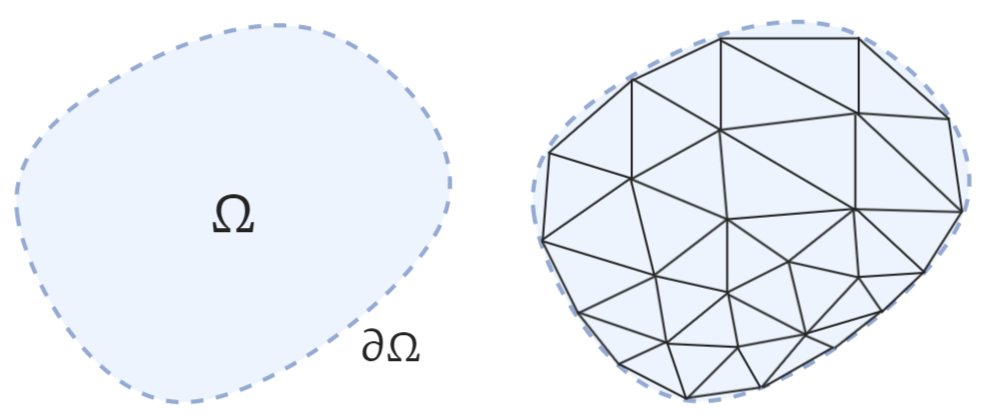
\includegraphics[width=\columnwidth]{FEM.PNG}
    \caption{Illustration of a Finite Element Method meshing. Here the discretization of a domain $\Omega$ with boundary $\partial \Omega$ into simpler polygons is shown.}
    \label{fig:FEM}
\end{figure}


\section{Current through a Carbon Nanotube Calculations}\label{Current Calculations}

Here we present a calculation to determine the feasibility of generating a magnetic field by passing a current through a carbon nanotube. Consider Ampere's Law:

\begin{equation*}
    \oint \Vec{B}\cdot \Vec{dl} = \mu_o I_{enc}
\end{equation*}

In other words, this expression tells us that the line integral of the magnetic field around any closed loop is equal to the permeability times the current enclosed in that loop. Note that this expression reduces to the following for an infinitely long cylinder:

\begin{equation*}
    B = \frac{\mu_o I_{enc}}{2\pi r}
\end{equation*}

We can compute the gradient of the magnetic field as follows:


\begin{equation*}
    \nabla B  = \big (  \frac{\partial \Vec{B}}{\partial r} \hat{r} \ , \ \frac{1}{r}  \frac{\partial \Vec{B}}{\partial \theta} \hat{\theta} \ , \ \frac{1}{r \sin(\theta)} \frac{\partial \Vec{B}}{\partial \phi} \hat{\phi}  \big )
    \newline
\end{equation*}
\begin{equation*}
    = \big (  \frac{\partial \Vec{B}}{\partial r} \hat{r} \ , \ 0 \ , \ 0  \big )
\end{equation*}

We require $G_m = | \nabla B | \sim 10^8 \ Tm^{-1}$ as described in \cite{project_paper}. Therefore:

\begin{equation*}
    | \nabla B | = G_m = \big | \frac{\partial \Vec{B}}{\partial r} \big | = \big | \frac{- \mu_o I_{enc}}{2 \pi r^2} \big |
\end{equation*}
\begin{equation*}
    \therefore \big | I_{enc} \big | = \frac{10^8 Tm^{-1} \cdot 2\pi (10^{-8}\ m)^2}{4\pi \cdot 10^{-7} \ Tm/A}
\end{equation*}
\begin{equation*}
    \big | I_{enc} \big | \sim 0.05 A \sim 10^{-1}\ A
\end{equation*}

Similarly, for $G_m = 10^7 \  Tm^{-1}$, we obtain $\big | I_{enc} \big | \sim 10^{-2}\ A$. We note that these are very large currents for nanoscale devices; it was reported in \cite{I_V_CNT} that typical nanoscale devices, and in particular carbon nanotubes, can have current on the order of $10^{-6}\ A$ going through them. Any current exceeding this threshold is bound to create adverse Joule-heating effects. As mentioned in \cite{project_paper}, we can relax $G_m$ to $10^6  \ Tm^{-1}$ for  masses on the order of $fg = 10^{-15} \ g$; however, these nanowires are on the order of $pg = 10^{-12}\ g$. Thus we conclude that generating a magnetic field by passing a current through the nanowire is likely unfeasible, and may lead to adverse heating effects in the resonator material if implemented. 

\section{Types of optomechanical resonators}\label{Types of optomechanical resonators}
Some of the most commonly used optomechanical resonators used experimentally are shown in Figure \ref{fig:optomechanical_devices} \cite{cavity_optomechanics_2014}.


\centering
\begin{center}
    \begin{figure}[htb]
    \centering
    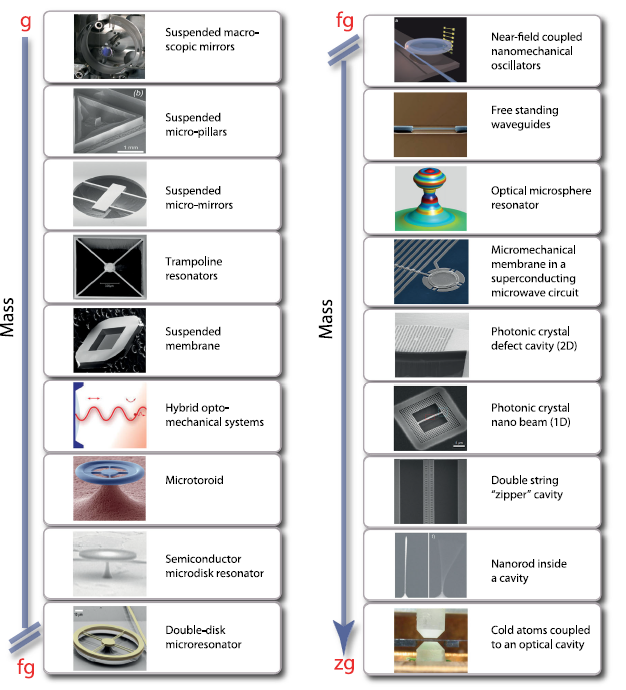
\includegraphics[width = \columnwidth]{optomechanical_devices.PNG}
    \caption{Optomechanical devices arranged according to mass (from \cite{cavity_optomechanics_2014})}
    \label{fig:optomechanical_devices}
\end{figure}
\end{center}


\section{List of optomechanical parameters}
\flushleft
Table \ref{tab:Optomechanical Parameters} lists some of the relevant optomechanical parameters used in this project. 



\begin{table*}[t]
    \centering
    \begin{tabular}{|c||c|c|}
    \hline
    Parameter & Description & Expression/Relation \\
    \hline
    
    $\Omega_m$ & Mechanical resonator frequency & - \\
    \hline
    $\Gamma_m$ & Mechanical damping rate & $\Gamma_m = \Omega_m / Q_m$ \\
    \hline
    $f_m$ & Mechanical oscillation frequency & $f_m = 2\pi/ \omega_m$ \\
    \hline
    $\omega_m$ & Mechanical angular frequency & $\omega_m = 2\pi f_m$ \\
    \hline
    $\omega_{cav}$ & Cavity resonance frequency & $\omega_m = 2\pi f_m$ \\
    \hline
    $m$ & Mass of mechanical resonator & - \\
    \hline
    $m_{eff}$ & Effective mass of resonator & See page \pageref{Vibrational Energy} \\
    \hline
    $\kappa$ & Photon dissipation rate & - \\
    \hline
    $Qf$ & Measure of the degree of decoupling & Require $Q_m f_m = Q_m \Omega_m /2\pi > k_B T / \hbar$ for neglecting \\ 
    & from the thermal environment  &  thermal decoherence over one mechanical period \\
    \hline
    $\kappa / \Omega_m$ & Sideband suppression factor.  & - \\
    & Determines the ability to realize ground state cooling.  & \\
    \hline
    $g_o$ & Bare optomechanical coupling rate & $\hat{H}_{int} = -\hbar g_o \hat{a}^\dagger \hat{a} (\hat{b}^\dagger + \hat{b} )$ \\
    \hline
    $g$ & Optomechanical coupling rate & $g = g_o \sqrt{\bar{n}_{cav}}$\\
    \hline
    $G$ & Optomechanical frequency shift per displacement & $G = \partial \omega_{cav} / \partial x$ \\
    \hline
    $x_{zpf}$ & Mechanical zero-point fluctuation amplitude & $x_{zpf} = \sqrt{\hbar / 2 m_{eff} \Omega_m}$ \\
    \hline
    $\hat{a}$ & Photon annihilation operator & $\hat{a}^\dagger \hat{a}$ is the photon number \\
    \hline
    $\hat{b}$ & Phonon annihilation operator & $\hat{b}^\dagger \hat{b}$ is the phonon number \\
    \hline
    $\bar{n}_{th}$ & Average phonon number in thermal equilibrium & $\bar{n}_{th} = \big ( e^{\hbar \Omega_m / k_B T} - 1 \big ) ^ {-1}$ \\
    \hline
    $\bar{n}_{cav}$ & Average phonon number in thermal equilibrium & $\bar{n}_{cav} = \langle \hat{a}^\dagger \hat{a} \rangle $ \\
    \hline
    $\gamma$ & Thermal decoherence rate & $\gamma \approx \Gamma_m \bar{n}_{th}$ \\
    
    \hline
    \end{tabular}
    \caption{Optomechanical Parameters \cite{cavity_optomechanics_2014}}
    \label{tab:Optomechanical Parameters}
\end{table*}




\newpage
% The \nocite command causes all entries in a bibliography to be printed out
% whether or not they are actually referenced in the text. This is appropriate
% for the sample file to show the different styles of references, but authors
% most likely will not want to use it.
\nocite{*}

\clearpage
% \begin{thebibliography}{}

% \bibitem{Project Paper}
% Ghobadi, R., Wein, S., Kaviani, H., Barclay, P. & Simon, C. Progress toward cryogen-free spin-photon interfaces based on nitrogen-vacancy centers and optomechanics. Physical Review A 99, (2019).

% \bibitem{Ghadimi}
% Ghadimi, A. H. et al. Elastic strain engineering for ultralow mechanical dissipation. Science 360, 764–768 (2018).

% % \bibitem{}

% \end{thebibliography}


\bibliographystyle{plainnat}
% \bibliographystyle{plain}
\bibliography{apsamp.bib}% Produces the bibliography via BibTeX.



\end{document}
%
% ****** End of file apssamp.tex ******
